\chapter{实验基础、理论模型和数值方法}\label{chap:chap2}


本作中将复杂力学环境简单的区分为 1. 自由环境;2.
自然边界(自由和固体平界面);3. 多空泡系统;4.
特殊声场环境。将复杂环境如此区分主要出于静、动态和作用尺度的考量。
空泡的注入以激光聚焦形成的能量沉积实现,以击穿机制形成空泡。
空泡的探测以高速摄像术和超短曝光时间阴影照相术为主。
为精密且简单的实现激光空泡所注入的不同复杂力学环境,提出了多种方法。
为对实验过程中涉及到的无法直接测量的参数和未能完全实现的情景进行研究,采用了基于求解
Navier-Stokes 方程的流场模拟研究。


\section{空泡动力学瞬态捕捉方法}

在本作中涉及到的探测方法为简单的阴影法。阴影法是通过将匀光准直后的照明光通过探测区域,经过当地密度变化改造光的传播方向,从而在成像面形成带有当地信息特殊图像的方法。
本例中,当空泡形成时,其阻挡照明光线的直线传播,从而使像形成明显的暗色区域,此即空泡的阴影。而激光击穿形成的冲击波在水中传播,压缩当地水体,使当地水体的折射率发生变化。通常阴影图的亮度与密度变化的二次导数成正比关系。当
$\frac {\partial ^2 n}{\partial ^2 x}>0$时,即
 $\frac {\partial ^2 \rho}{\partial ^2 x}>0$时,光线发散,形成暗区。而
$\frac {\partial ^2 n}{\partial ^2 x}<0$时,即
$\frac {\partial ^2 \rho}{\partial ^2 x}<0$
时,光线汇聚,有可能形成高亮区域。但因为其对二阶导敏感,通常难以用于定量的分析,在空泡研究领域一般用于追踪空泡边界和冲击波的波前。而背景光照相法,通过调节成像镜头的成像位置,也可以获得空泡的阴影图像。
激光击穿后,形成的冲击波和非液相物质边界的移动速度在其初期可以达到
1500m/s,后续减速直到最大泡半径。后续溃灭的速度也能达到 1000m/s
量级。为了对该高速过程进行瞬态的形态捕捉,设计了单帧瞬态曝光照相系统(Single
Frame Transient Exposure Photography,SFTEP)。 SFTEP
是指将暗室相机打开采集,在采集期间将击穿激光入射并致空泡形成,然后在特定的空泡阶段入射短脉宽照明脉冲,照明脉冲携带路径上的信息使相机采集器曝光。其更清晰的时序如图\ref{fig2.1}
所示。更具体的曝光阶段由等离子体闪光和照明光的时间差获得。此相对时间获得方法可以减少激光器受触发信号出光时间不稳定造成的时间波动。
SFTEP
优势在于,通过控制照明脉冲的脉宽,获得超短曝光时间,以获得清晰的相变边界。如本作中使用
2.5ns 的脉宽,在冲击波传播初期,在曝光周期内,冲击波波前只移动了
$2.5*10^{-9}\mathrm s*1.5*10^3 \mathrm {m/s}=3.75*10^{-6}m$,
这个值在图像上通常小于一个像素。SFTEP
能够采用较为廉价且简单的设备获得极为精准的瞬态捕获。

\begin{figure}[h]
\centering
\includegraphics[width=0.9\linewidth]
%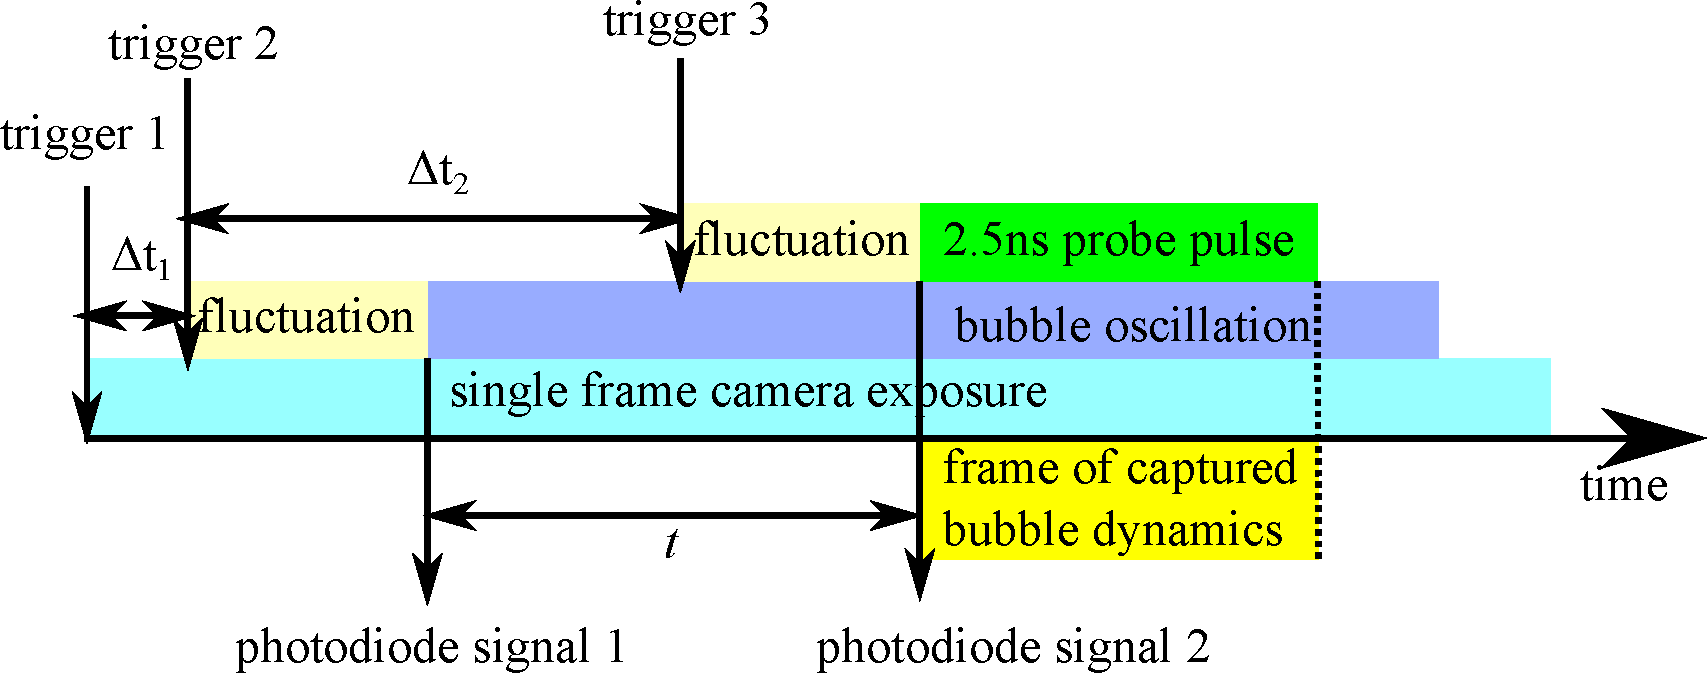
\includegraphics[bb=00 00 200 100]
{img/fig2.1-eps-converted-to.pdf}
\caption[单帧曝光瞬态照相系统时序图]{单帧曝光瞬态照相系统时序图。}
\label{fig2.1}
\end{figure}


通过高速摄影机和背景光照相方法可以更简单的获得连续的空泡脉动全过程。通过超高速摄像机和飞秒脉冲照明正逐渐成为微纳流体领域的标准配置。在本作中采用较为传统的连续白光照明,和短曝光时间的高速摄像机结合的方法。其曝光时序图如图\ref{fig2.2}
所示。这里超高速摄像机采用的是固定曝光触发方式:其内部产生一个固定的曝光时序,其曝光时间差可程序控制,在开始工作后,一直记录当前收到的图像,并循环存放在超高速缓存中,在收到触发信号后,摄像机记录触发时间,并将拍摄的内容保存进内存而后电脑中。

\begin{figure*}[h]
\centering
\includegraphics[width=0.9\linewidth]
%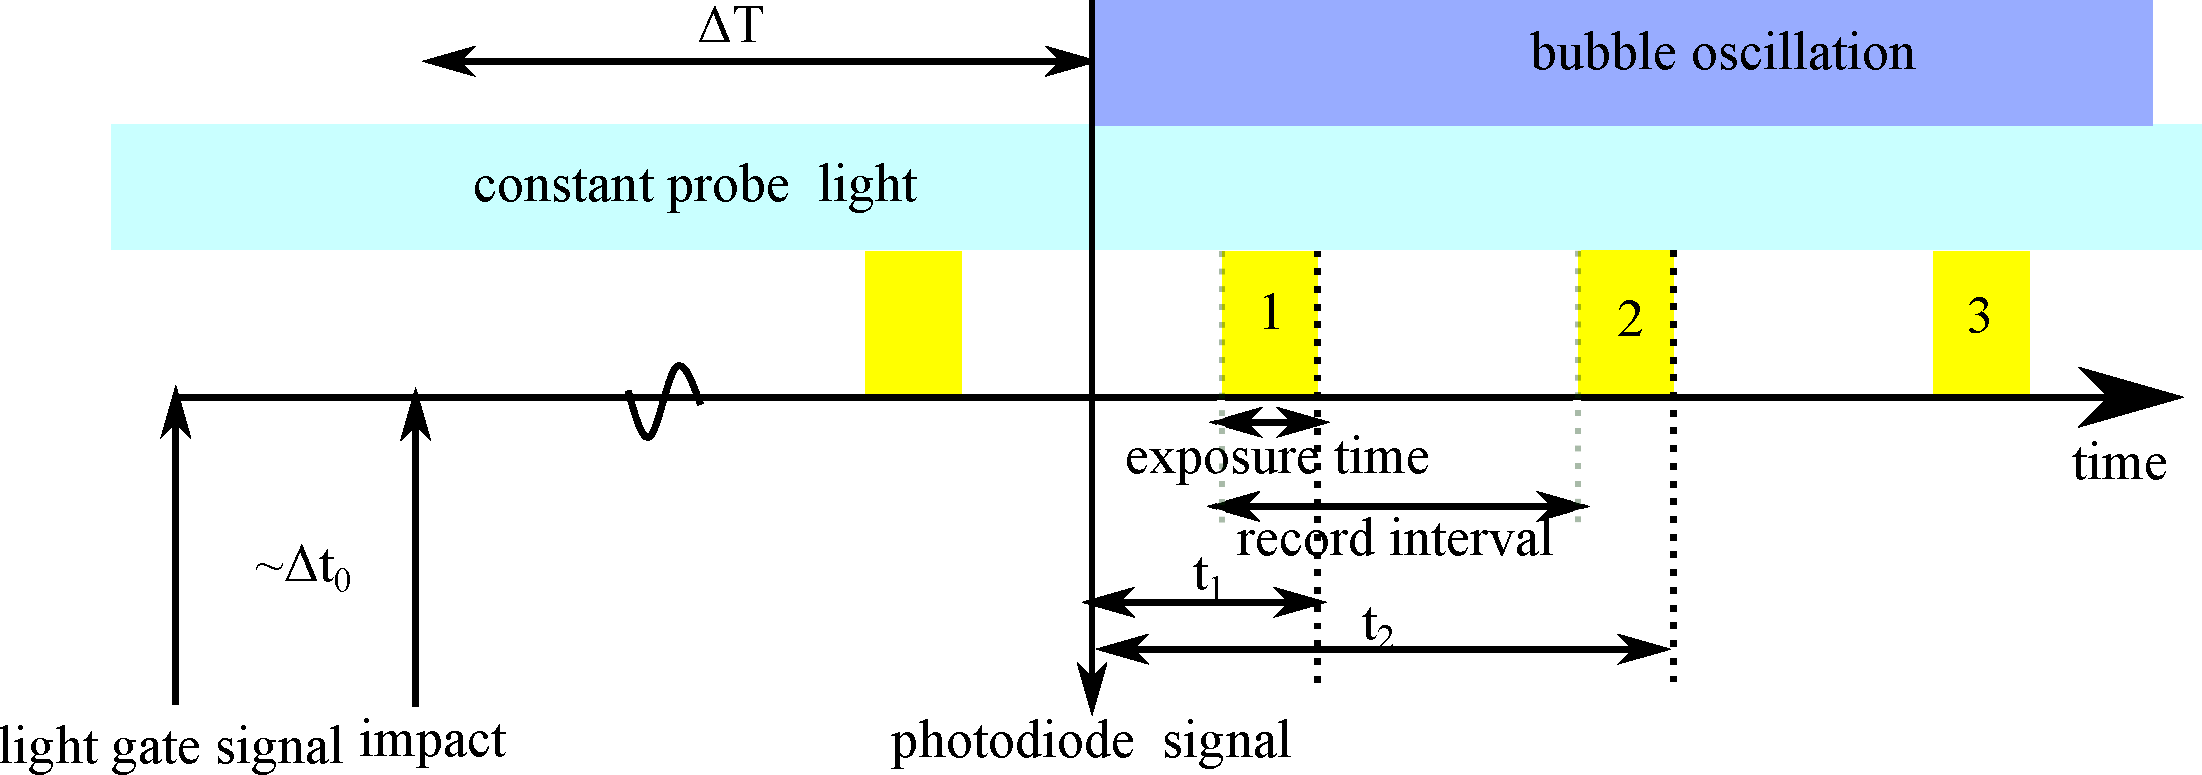
\includegraphics[bb=00 00 400 400]
{img/fig2.2-eps-converted-to.pdf}
\centering
\caption[高速摄像机曝光时序图]{高速摄像机曝光时序图.}
\label{fig2.2}
\end{figure*}



\section{激光致球形空泡的引入}

激光的单色性较好,在实验中通常不计其聚焦时存在的色差,且等离子激发激光通常是平行近轴入射,一般认为,透镜导致激光聚焦时形成的球差能导致空泡起始状态的不规则形状。如下是使用
 $\mathrm {arctan}(5\mathrm {mm}/20\mathrm {mm})\approx 24.5^{\circ}$
聚焦角度的透镜获得的击穿等离子闪光区域。该图\ref{fig2.3}通过三十次独立曝光加总获得。该等离子体形状符合张冲等\cite{zhang_transient_2016}前序研究模型所预言。通过普通透镜击穿获得的空泡,具有明显的长短轴的区分,在光轴方向上具有更长的击穿长度,在除前后尾端外的主体部分,光轴更靠近光入射方向的区域具有相对较大的击穿宽度。在等离子复合熄灭后,进入热力学和流体力学主导的过程后,此时视作空泡起始状态。空泡的膨胀初期首先要在垂直与光轴方向上膨胀,由此会形成一个初期主轴沿着光轴方向,膨胀后形成主轴垂直与光轴的如此一个光轴转置的过程,在空泡的球性上较弱。通常在领域内,由此以初始形状的曲率预测空泡脉动拓扑变化。


\begin{figure*}[h]
\centering
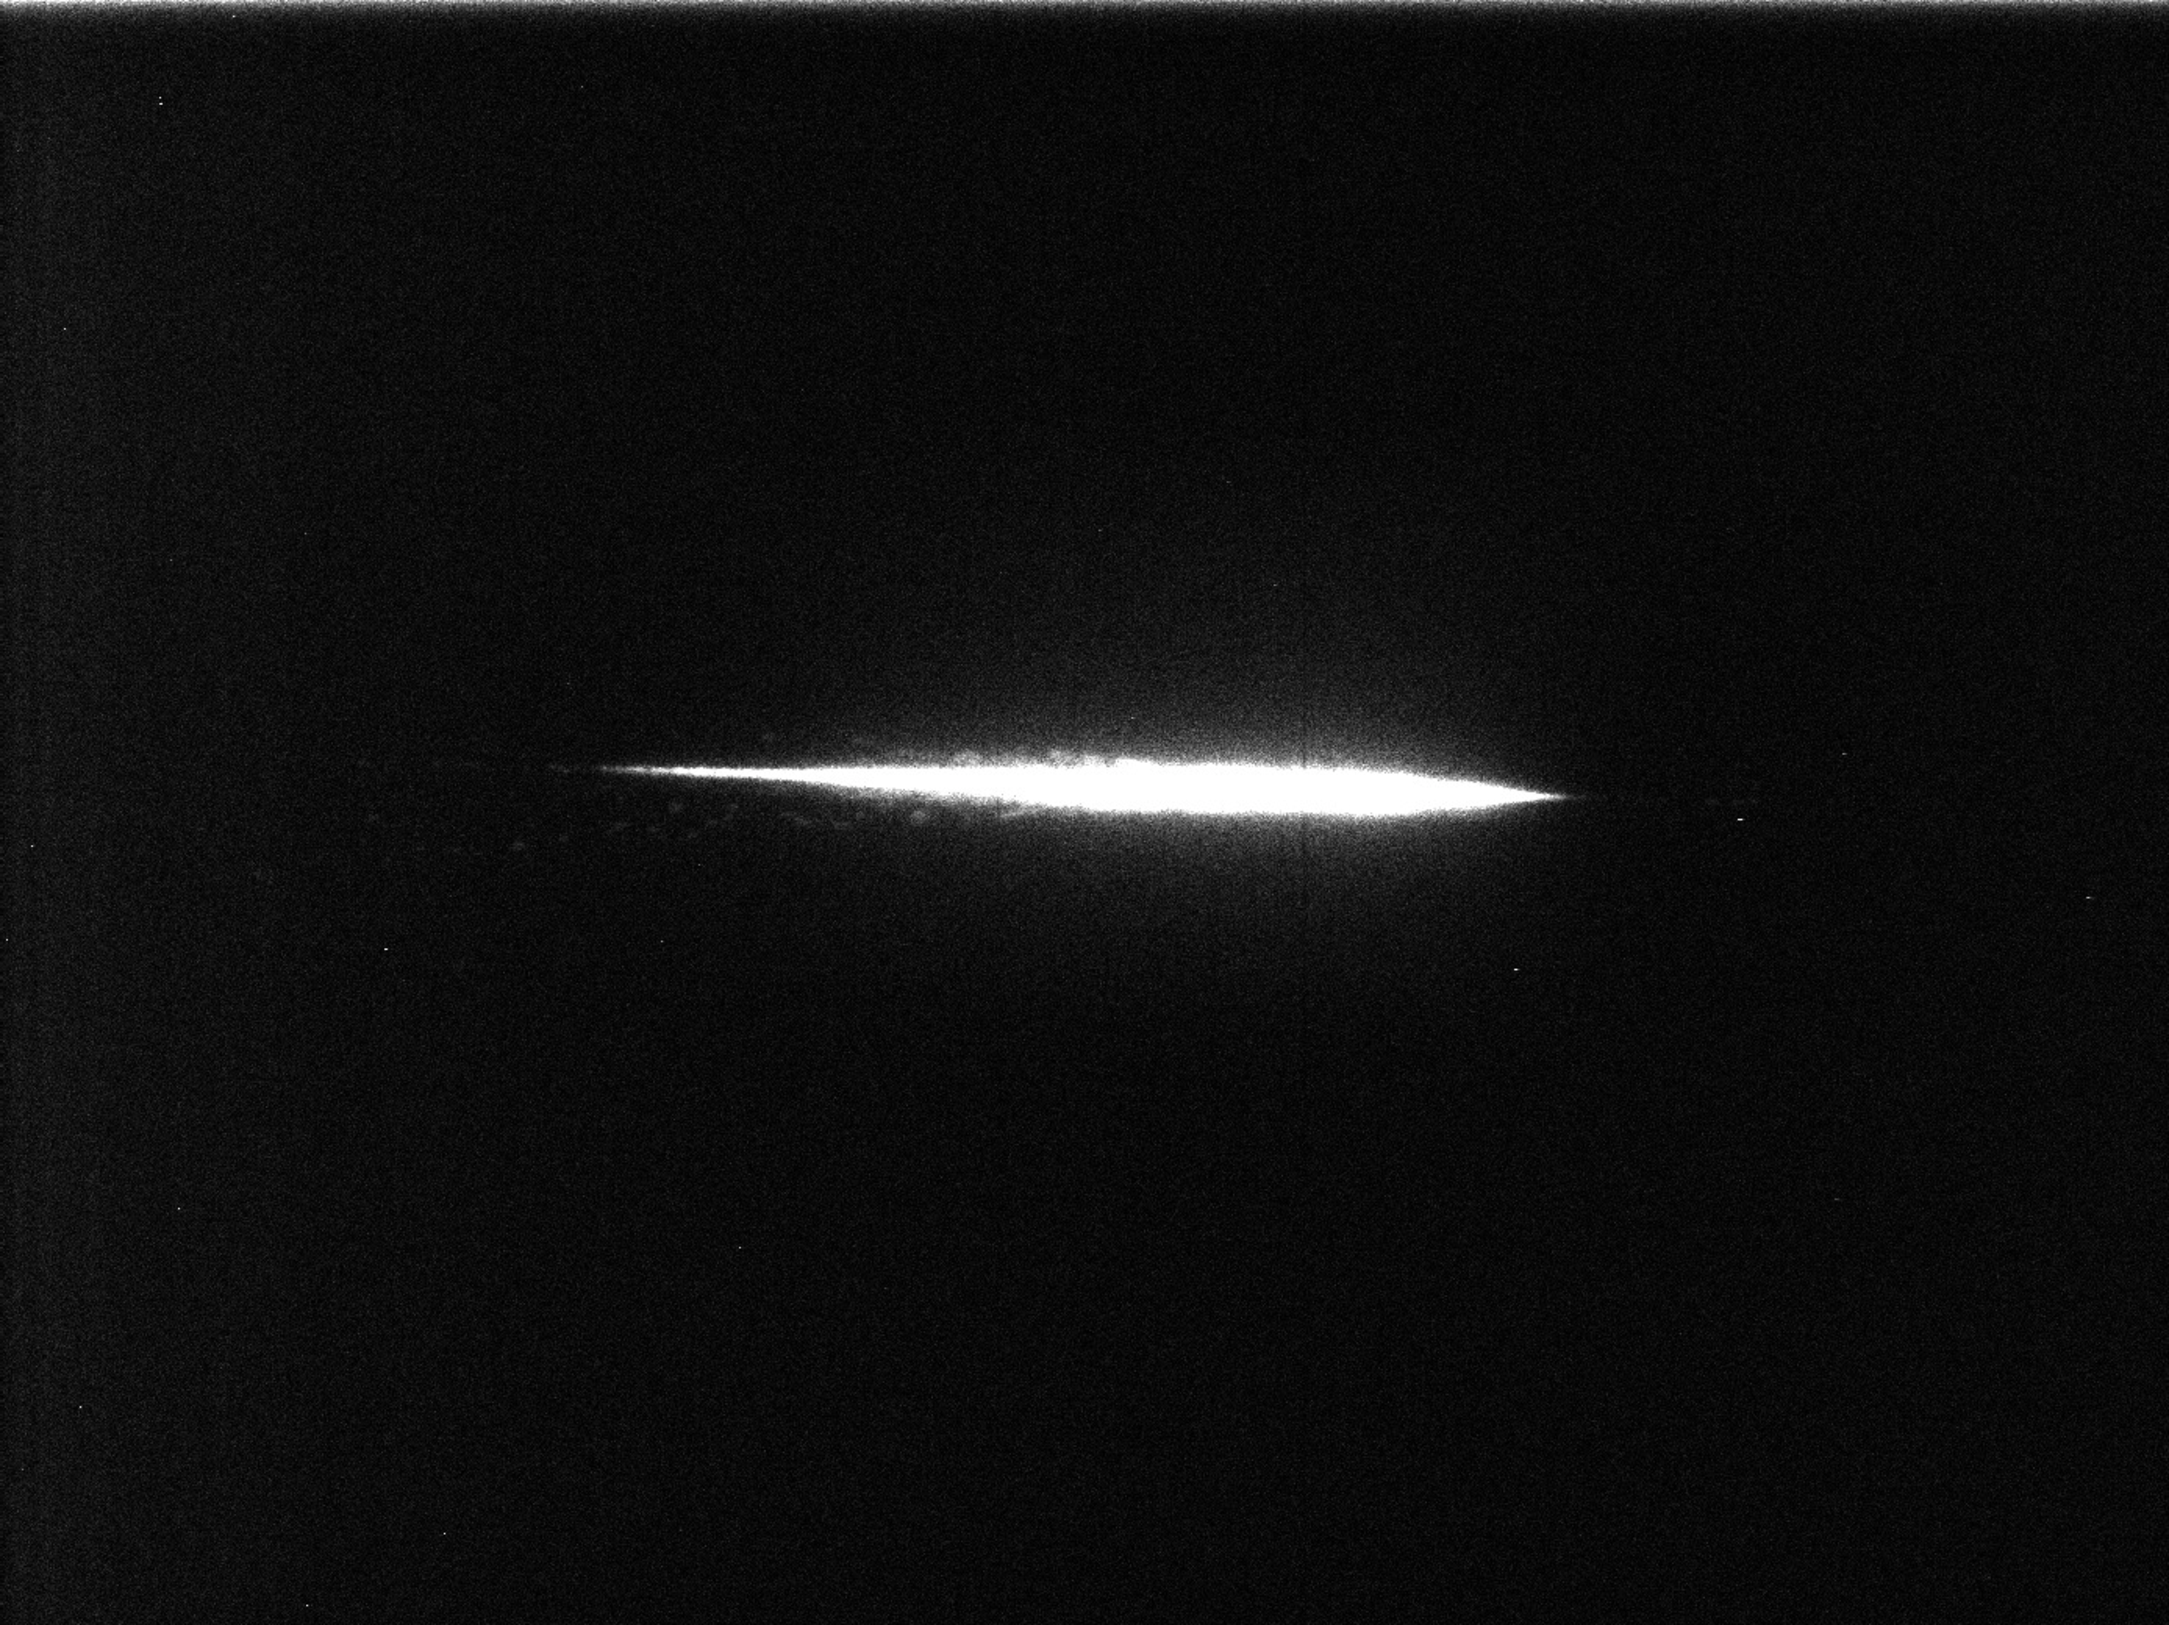
\includegraphics[width=0.5\linewidth]{img/fig2.3-eps-converted-to.pdf}
\centering
\caption[激光击穿致等离子体闪光]{激光击穿致等离子体闪光。闪光区域通过三十次独立的击穿闪光曝光加总获得。}
\label{fig2.3}
\end{figure*}



\begin{figure*}[h]
\centering
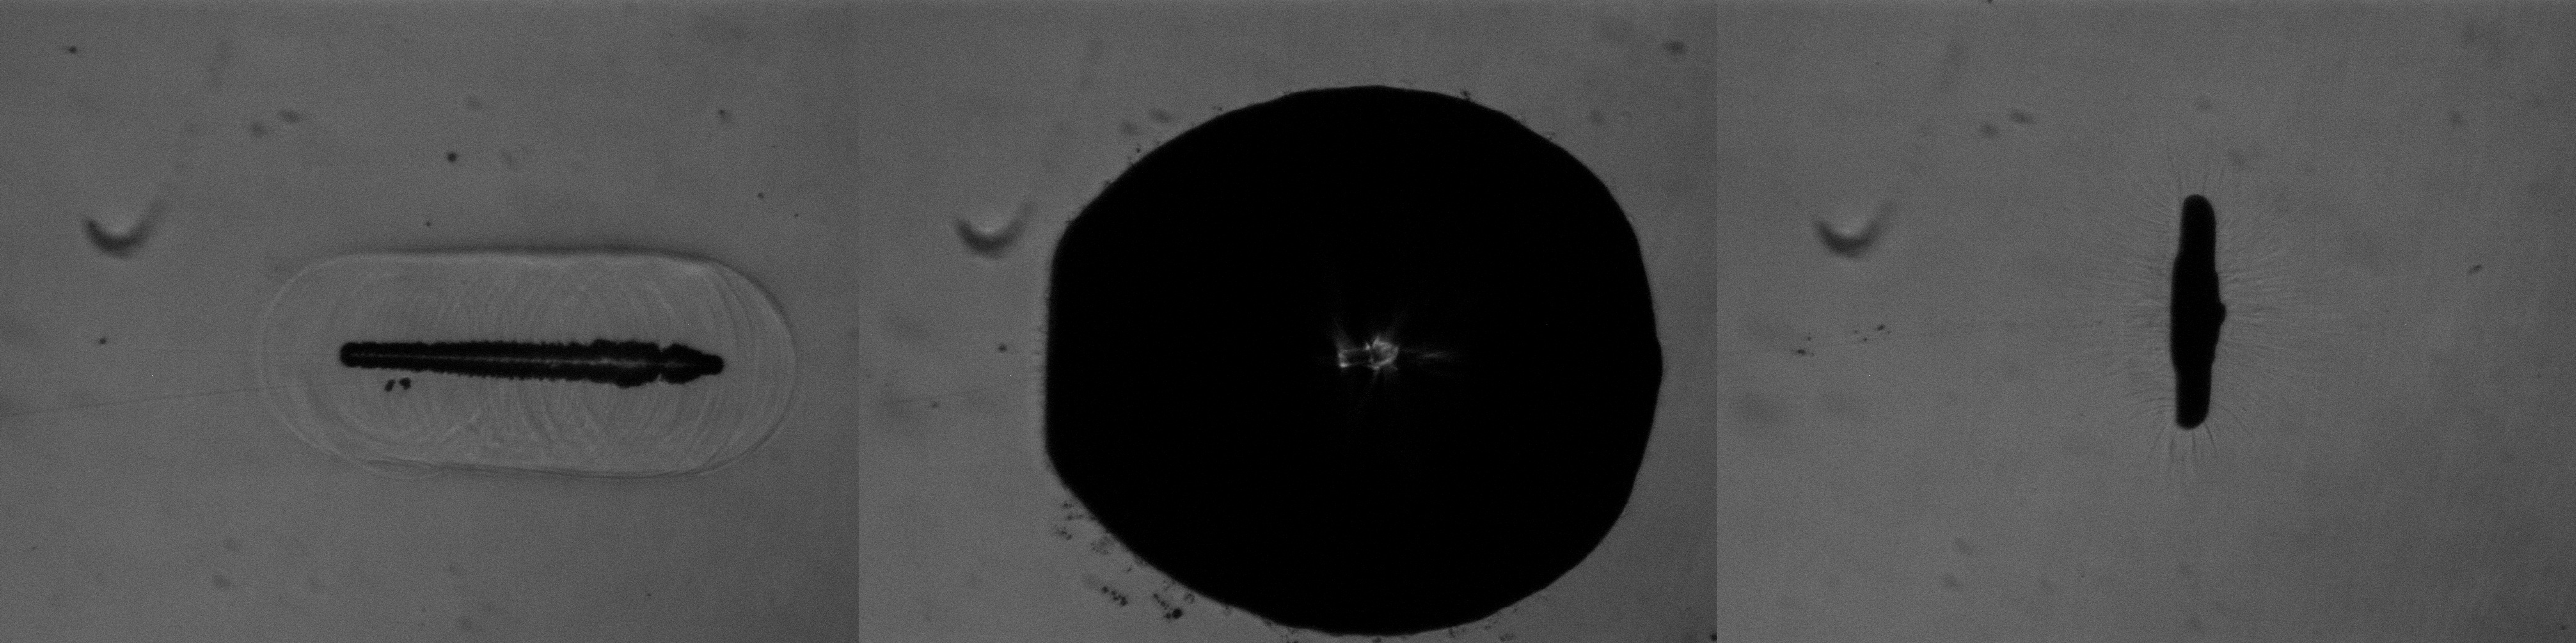
\includegraphics[width=0.7\linewidth]{img/fig2.4-eps-converted-to.pdf}
\centering
\caption[多点击穿/超长聚焦击穿形成的空泡及溃灭]{多点击穿/超长聚焦击穿形成的空泡及溃灭。}
\label{fig2.4}
\end{figure*}


这种普通透镜因球差导致多点击穿的现象,可以通过多种方法克服。最常用的方法是提高聚焦角的角度大小。在激光击穿致空泡的相关研究中,一般认为聚焦角大于
$29.8^{\circ}$ 时,可以忽略其多点击穿现象,而只认为其为点状击穿
\cite{fu_experimental_2018}。其次是通过加大激光脉冲能量,使其膨胀至最大泡半径时,其泡半径远大于多点击穿区域长度。这种方法往往受限于激光器性能。再次是减弱激光能量,使其在原击穿区域无法形成击穿,从而认为其是点状击穿。此时形成的空泡尺寸较小,需要通过更加激进的探测方法来获得其动力学特征。
而在实际实践中,更加技术的选择是:1. 通过显微物镜聚焦击穿。2.
通过双胶合消像差透镜击穿。3.
通过凹面镜反射击穿。显微物镜方案成熟,对平行光的聚焦能力好。而双胶合消像差透镜能承受较大脉冲能量。凹面镜成本较高,且对空泡所在水域形成边界改造。在本作中,选用显微物镜击穿方案和双胶合消像差透镜击穿方案。\\
在本作中涉及到的分束镜片(Diffractive Optical
Element,DOE)是一种基于光波衍射理论,利用微纳刻蚀方法,设计制造的一种具有特殊表面结构,能够对光波前位相分布进行精细调控的光学元件。

\begin{figure*}[h]
\centering
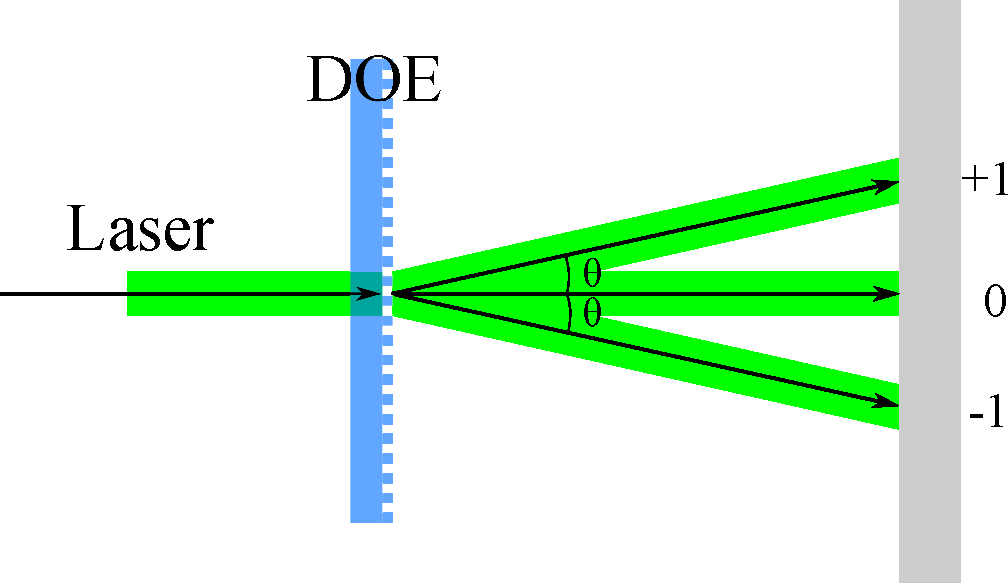
\includegraphics[width=0.5\linewidth]{img/fig2.5-eps-converted-to.pdf}
\centering
\caption[DOE
衍射分波片示意图]{DOE衍射分波片示意图。}
\label{fig2.5}
\end{figure*}



通常衍射分束镜片将准直光束分为一维(二维)排列的多个光束,每个光束保持原来的特征,以不同的角度出射。衍射分束器本质上是光栅结构,其出射角满足光栅方程。通过精心的设计二元或多元的衍射单元结构,可实现各路输出之间的能量分配。一维或二维阵列光束,通过透镜聚焦后可形成焦点阵列,用于高功率激光并行加工。

\begin{figure*}[h]
\centering
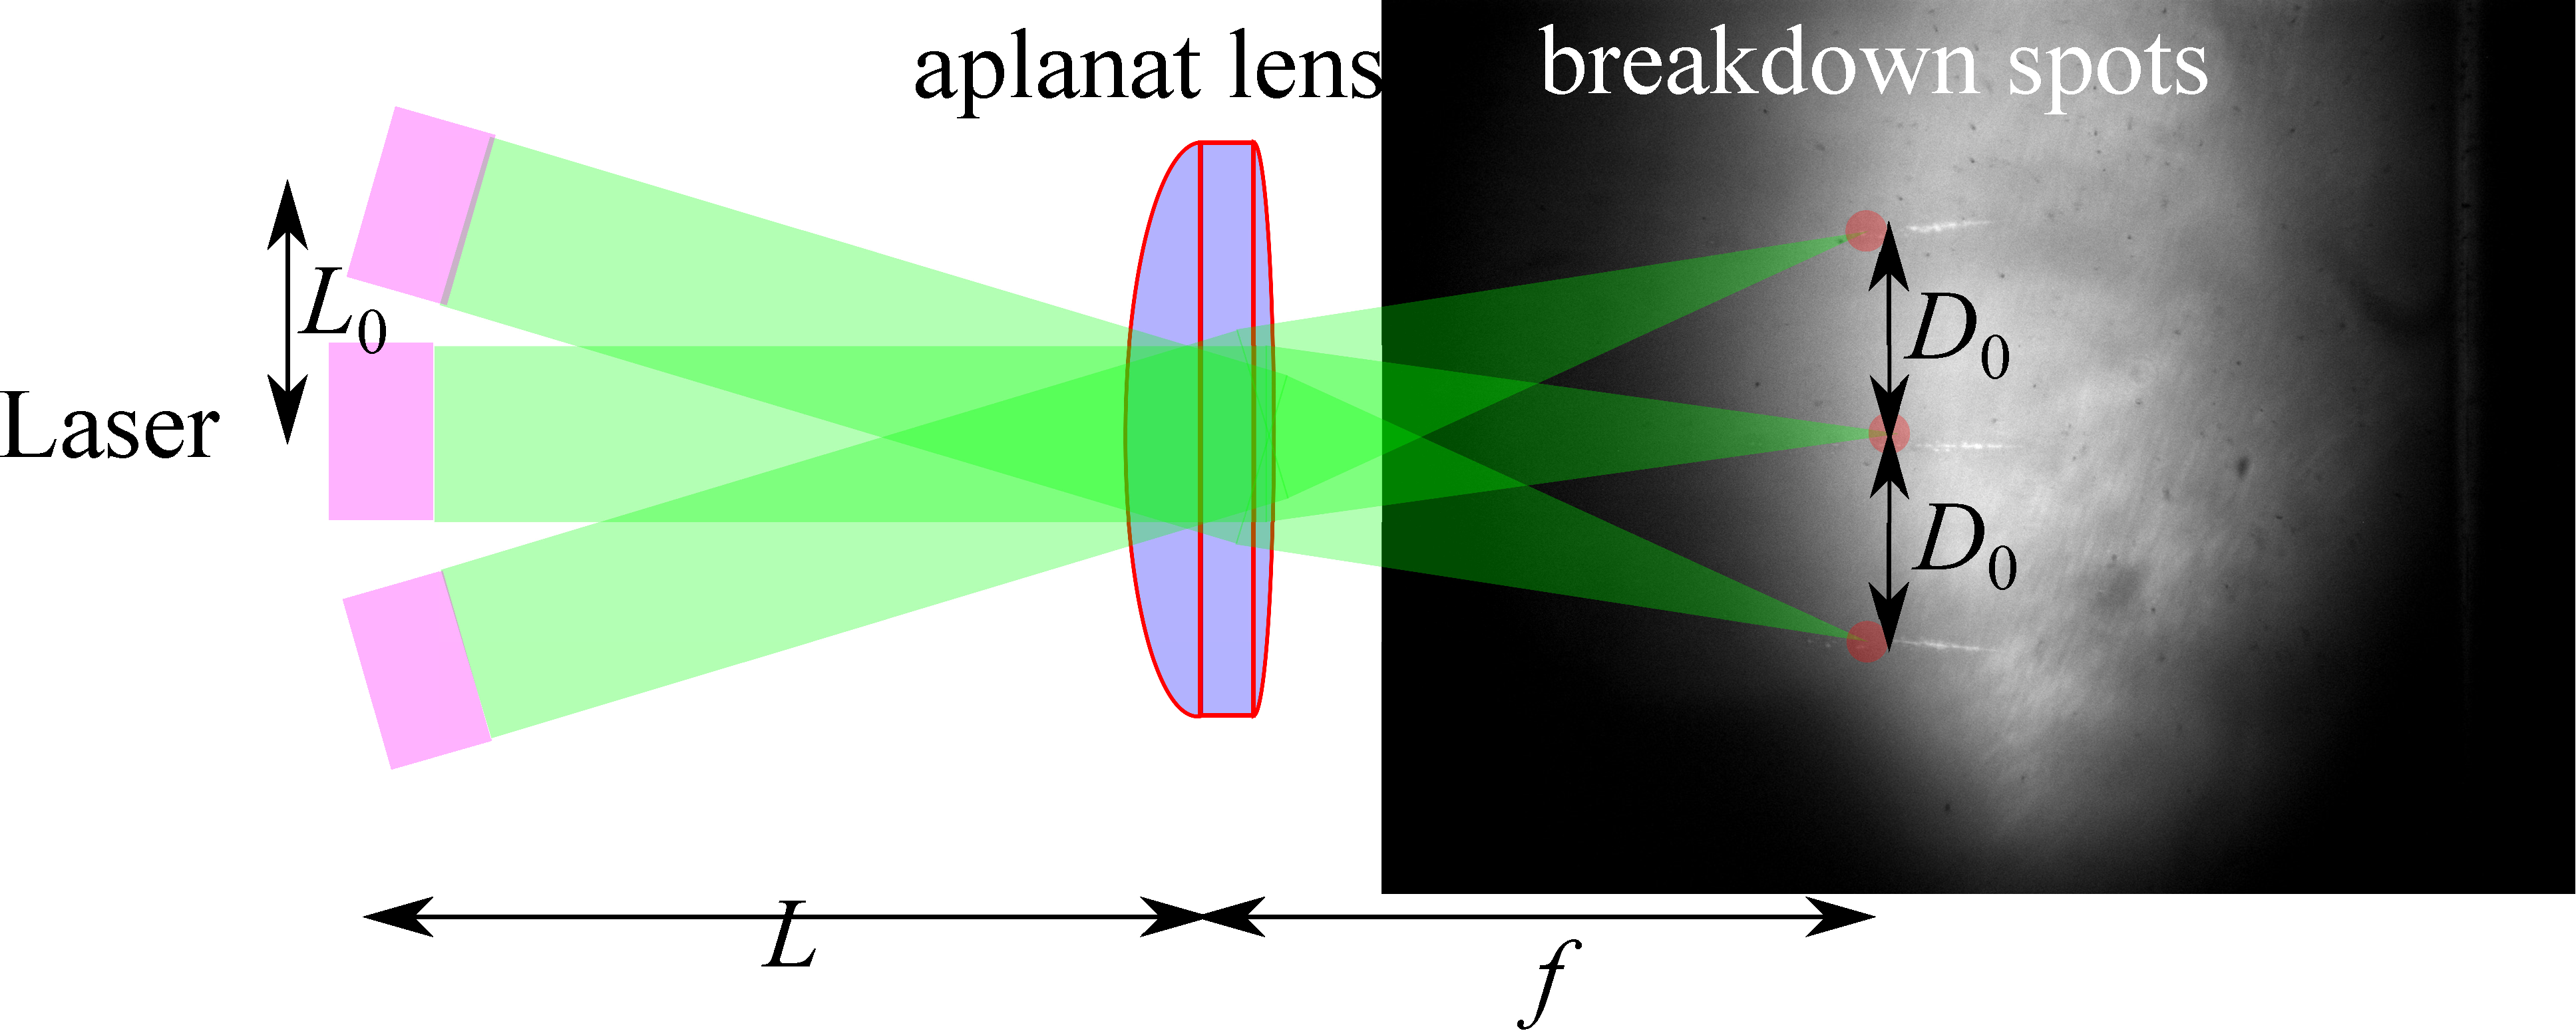
\includegraphics[width=0.6\linewidth]{img/fig2.6-eps-converted-to.pdf}
\centering
\caption[DOE分束光反射聚焦击穿示意图]{DOE分束光反射聚焦击穿示意图。}
\label{fig2.6}
\end{figure*}



在本作第四章的实验方案中,通过 DOE
分束后用反射镜将反射激光反射进聚焦透镜,激光在透镜焦平面击穿,如图\ref{fig2.4}
所示。其中可控制的击穿点距离满足如下关系: 
\begin{equation}
    D_\mathrm 0=\frac {f L_\mathrm{0}}{L} \,。
    \label{2.1}
\end{equation}


 通常将光分束后 $L_\mathrm{0}$
不易改变,实验中采用分体式可移动击穿和探测装置,以便于调节
$L$,从而获得不同 $D_\mathrm 0$。

\section{撞击致压力波的引入}\label{ux649eux51fbux81f4ux538bux529bux6ce2}


\begin{figure*}[h]
\centering
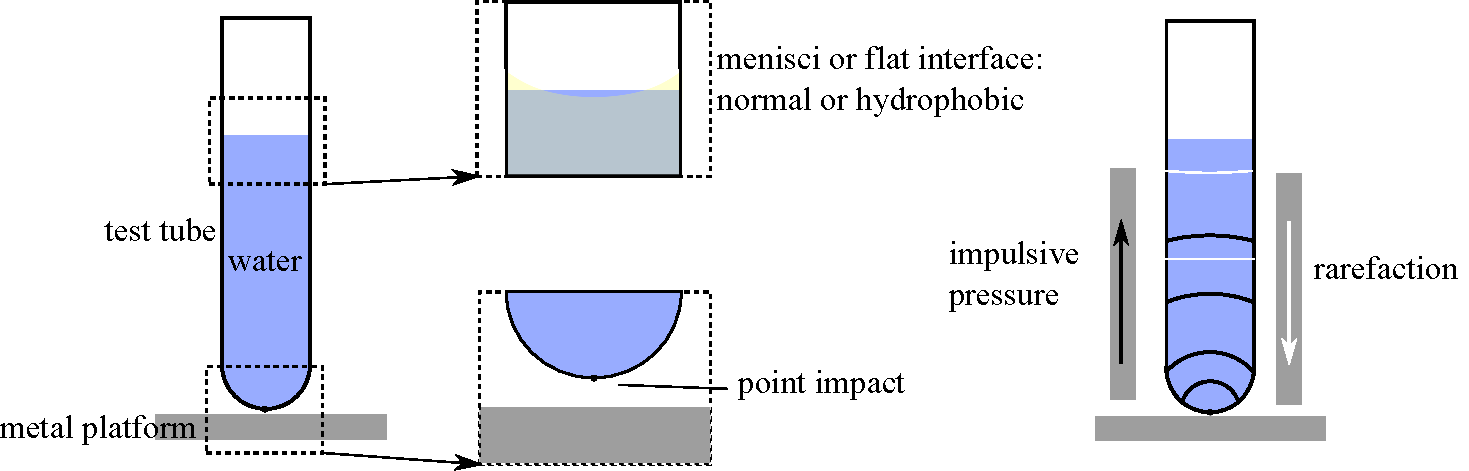
\includegraphics[width=0.9\linewidth]{img/fig2.7-eps-converted-to.pdf}
\centering
\caption[试管撞击产生压力波]{试管撞击产生压力波。本文中忽略事实上存在的张力致毛细曲面。且认为撞击产生的压力波为平面波。}
\label{fig2.7}
\end{figure*}


为了简单的获得压力波,本文利用试管的球形底面撞击硬质金属平面产生冲击压力波。这个方法在上个世纪被提出,最近五年重新受到关注。为了清楚和简单起见,我们对撞击产生的压力波采用一维平面波模型,忽略试管球底形状和液体与空气的界面因亲水性形成的曲面,并有以下假设:(i)管子的横截面积在整个传播方向上是恒定的;(ii)管壁是刚性的;(iii)声波是线性的;(iv)介质是无粘性的。
流体与管壁相互作用的程度可以用无量纲参数''流体负荷''
$\beta=(c_l^2/c_s^2)(\rho _l/\rho_s)(2R)/h$ 
来量化\cite{shepherd_shock_2010}。
其中 c 项是纵向声速比,$\rho$项是密度比,最后一项是尺寸比。下标 l 和s分别表示液态和固态相。在本文特殊的例子中,我们有$\beta\approx2.25e-5<<1$,表明了液体和试管的弱耦合性。从而本作中只将其撞击点作为压力波源考虑,而忽略其压力波在刚体壁面传播再回馈到液体中的部分。且由于本文中涉及的撞击是在低速下产生的,几巴甚至几百巴的压力扰动是在线性声学理论的有效范围内的\cite{dynamics_applied_nodate}。由于假设
(ii) 和 (iii) 的结果,预计声波在管内将以液体中的声速传播。
声波在介质中传播,本质是介质偏离平衡态的扰动的传播。而为了让介质位移需要克服介质内存在的阻力,这种阻力通常称为声阻抗(
acoustic impedance, $Z$)。其一般用下式表示:
\begin{equation}
    Z=\rho c
\label{2.2}
\end{equation}

其中 $\rho$ 为介质密度,$c$ 为介质的本地声速(纵向)。
压力波动在传播过程中,如遇到两种不同声阻抗物体所构成的声学界面时,一部分波动会反射到前一种介质中;另一部分波动在进入第二种介质时发生传播方向的改变,即折射。波的反射压强可以根据声阻抗进行量化,其主要取决于界面两旁的两种介质的声阻抗差值
(入射方介质 $Z_1$,和透射方介质 $Z_2$),其符合如下关系:
\begin{equation}
p_{\mathrm{ref}}=\frac{Z_{\mathrm{2}}-Z_{\mathrm{1}}}{Z_{\mathrm{2}}+Z_{\mathrm{1}}}p_{\mathrm{inc}}\\ \,,
    \label{2.3}
\end{equation}

一般声阻抗差值越大,反射强度越大,反之则小。在极端情况下,入射波从非常坚硬的材料到柔软的材料(例如,液体到气体,
$Z_l>>Z_g$
),反之(例如,液体到固体,$Z_l<<Z_s$),声学关系变得非常简单。如果液体中的波与气液界面发生碰撞,则波向气体方向的传输是如此之小,以至于界面上的压力几乎保持不受干扰(即自由边界)。而因空气的声阻抗远小于水的声阻抗,故而在自由界面产生的声反射形成相位转换,也就是压力波在界面处反射形成舒张波。
由此,我们可以认为,在试管中任意一点,至少是中心轴上的点,其受到撞击形成的平面线性压力波和反射形成的舒张波作用,其压强值决定于压力波和其在顶部自由面反射形成的多次舒张波以及舒张波在底部刚面反射形成的多次压力波共同决定。

%
\section{空泡动力学的理论模型}


\subsection{Rayleigh-Plesset
模型}

如本作第一章中所介绍的,用于描述空泡脉动的物理模型非常多,有数学的,有经验的。下面给出
Rayleigh-Plesset 模型的推导。
典型的空泡内部充斥着水蒸气或者其他气体。由于表面张力的作用,空泡内部的压强一般高于环境水压。液体的表面张力系数($\sigma$)指每单位面积上的表面自由能。对一个理想的自由域内半径为
$R$ 的空泡,其表面能为 $4\pi R^2 \sigma$。空泡膨胀半径至 $R+d R$
时,其表面积变为
$4\pi (R+\mathrm{d}R)^2=4\pi R^2+8\pi R\mathrm{d}R$(忽略高阶项)。由此,空泡需要克服外界压力做功的力为
$8\pi R\sigma$。空泡内外压做功的平衡可做如下表示:$4 \pi R ^ { 2 } p _ \mathrm{ i n } = 4 \pi R ^ { 2 } p _ \mathrm{ B } + 8 \pi \sigma R$。其中
$p_\mathrm{in}$ 指泡内压, $p_\mathrm{am }$
指泡面压。于是可以获得如下关系:
\begin{equation}
    p_{\mathrm {in }}=p_{\mathrm {B}}+\frac{2 \sigma}{R} \,,
    \label{2.4}
\end{equation}

 式中右边第二项被称为"Laplace pressure"。水在 $20^\circ C$
时的表面张力系数
$\sigma=0.7275\,(\mathrm{N/m=J/m^2})$。空泡半径越小这个压力越大,在百纳米尺度可以达到
$10bar$ 以上,而在毫米空泡,相比外界水压,可以忽略。
空泡在脉动时,其周围的液体也会随着空泡运动。考虑一个半径为 $R_L$
的球状液体体积,其与具有实时半径 $R$ 的理想球形空泡同心。具有半径 $r$
和厚度 $\mathrm d r$ 的球壳有如下动能:
$1 / 2 \times 4 \pi r ^ { 2 } \rho_ { 0 } \mathrm d r \times ( \mathrm d r / \mathrm d t ) ^ { 2 }$
(质量和速度平方积的一半)。其中 $\rho_0$
是水的静止密度。这个体积的总动能是上式自 $R$ 到 $R_\mathrm L$
的积分: 
\begin{equation}
    E_\mathrm{K} =\frac{ 1 }{ 2 } \rho_{ 0 } \int_{ R } ^ {R_\mathrm{L}} (\frac{\mathrm d r } { \mathrm d t })^ 2 4\pi r^2 \mathrm d r = 2 \pi\rho_0 R^3 ( \frac{ \mathrm d R }{ \mathrm d t } )^2   \,,
    \label{2.5}
\end{equation}
 
 此处假设液体不可压缩,即
$4 \pi r ^ { 2 } \frac {\mathrm d r } {\mathrm d t } = 4 \pi R ^ { 2 } \frac { \mathrm d r } { \mathrm d t }$,且
$R<<R_\mathrm{L}$。
当空泡膨胀,其对环绕它的液体做功,当空泡溃灭,环绕液体对空泡做功。也就是空泡对环绕液体作负功。空泡对环绕液体做功可以表示为:
\begin{equation}
W _ \mathrm{ b u b b l e } = \int _ {R_\mathrm{0} } ^ { R } 4 \pi r ^ { 2 } p _ { B } \mathrm d r\,, 
\label{2.6}
\end{equation}

此处 $R_\mathrm{0}$
指气泡未受扰动时的初始半径,此处也指空泡的均衡半径。当空泡膨胀时,我们考虑的液体球壳体积也膨胀。也就是说液体球壳对环绕液体做功。当空泡溃灭时,这个液体球壳也收缩,并对环绕液体作负功。这个功可以表示为:
\begin{equation}
W _ \mathrm{ liquid } = p _ {\infty } \Delta V = p _ { \infty } N\int _ { R_ 0 } ^ { R } 4 \pi r ^ { 2 } \mathrm d r \\\,
    \label{2.7}
\end{equation}

 此处,$p _ {\infty }$ 是指环境静压。$\Delta V$
是空泡膨胀所排开的液体体积,由于不可压假设,也就是空泡变化的体积。
由能量守恒可得:
\begin{equation}
W _ { b u b b l e } = E _ { K } + W_\mathrm{liquid}\\\,
    \label{2.8}
\end{equation}

接下来对上式\ref{2.8}求对 $R$ 的微分。首先求式\ref{2.6}的微分: 
 
\begin{equation}
\frac { \partial W _\mathrm{bu  b b l e} } { \partial R } = 4 \pi R ^ { 2 } p_\mathrm B,
    \label{2.9}
\end{equation}

其次,求式\ref{2.5}的微分: 
\begin{equation}
\frac { \partial E _ { K } } { \partial R } = 6 \pi \rho _ { 0 } R ^ { 2 } ( \frac { \mathrm d R } {  \mathrm d t } ) ^ { 2 } + 4 \pi \rho  _ { 0 } R ^ { 3 } \frac {  \mathrm d ^ { 2 } R } {  \mathrm d t ^ { 2 } }\\\,
    \label{2.10}
\end{equation}

 并使用如下关系: 

\begin{equation}
\frac { \partial } { \partial R } [ ( \frac { \mathrm d R } { \mathrm d t } ) ^ { 2 } ] = \frac { \partial ( \dot{R} ^ { 2 } ) } { \partial R } = \frac {1} {\dot{R}} \frac {\partial ( \dot{R} ^ { 2 } )} { \partial t } = 2 \ddot R = 2 \frac { \mathrm d ^ { 2 } R } { \mathrm d t ^ { 2 } },
    \label{2.11}
\end{equation}

牛顿微分表示法中,$R$ 上标的点表示时间导数
$\mathrm d / \mathrm d t$,此处 $\dot{R}$, 是空泡壁面移动速度,
$\ddot{R}\,$ 是空泡壁面的加速度。 最后,式\ref{2.7}的微分:
\begin{equation}
\frac { \partial W_\mathrm{liquid }} { \partial R } = 4 \pi R ^ { 2 } p _ { \infty } \\\,
    \label{2.12}
\end{equation}


 将式\ref{2.9}, \ref{2.10}, \ref{2.12}代入,式\ref{2.8}对 $R$ 的微分表示为:

\begin{equation}
\frac { p _ { B } - p _ { \infty } } { p _ { 0 } } = \frac { 3 } { 2 } \dot R ^ { 2 } + R\ddot R ,
    \label{2.13}
\end{equation}

 空泡壁运动时,式 \ref{2.4} 中应包含额外的粘性项: 

\begin{equation}
p _ \mathrm { B } = p _ \mathrm { g } + p _ \mathrm { v } - \frac { 2 \sigma } { R } - \frac { 4 \mu \dot R } { R }\\\,
    \label{2.14}
\end{equation}
 此处 $p _ \mathrm { g }$,$p _ \mathrm { v }$
是不凝气体和水蒸气的分压,即
$p_\mathrm {in }=p _ \mathrm { g } + p _ \mathrm { v }$。而 $\mu$
是液体粘度。其中粘性项是通过不可压缩假设下,
$2\mu \frac { \partial \dot r } { \partial r } | _ { r =R }$ 获得。
最后,将式 \ref{2.14} 代入到式 \ref{2.13}中,可以推导出所谓的 Rayleigh--Plesset
公式:

\begin{equation}
R \ddot R + \frac { 3 } { 2 } \dot R ^ { 2 } = \frac { 1 } { \rho _ { 0 } } [ p _ { g } + p _ { v } - \frac { 2 \sigma } { R } - \frac { 4 \mu \dot { R } } { R } - p _ { 0 } - p _ { s } ( t ) ] 
    \label{2.15}
\end{equation}
 
 此处
$p_{\infty}=p _\mathrm { 0 } + p _\mathrm { s } ( t )$,$p_0$
是净液压,$p_\mathrm{s }$
是波长远大于空泡尺寸的声压。由于采用了不可压假设,其不适用于空泡溃灭速度达到当地声速时的情景。
\medskip
\bigskip

\subsection{考虑压缩性的 Keller-Miksis
模型}

而本文中采用的 Keller-Miksis
模型是描述单球形空泡脉动的一个更加完善的模型,其是当前学界普遍采用的数学的物理模型。它考虑了表面张力,粘性,可压缩性和空泡内容气体\cite{lauterborn_cavitation_1997,Brennen2003,keller_bubble_1980}。考虑一阶
1/C 时间延迟的等效模型写作:

\begin{equation}
    \left(1-\frac{\dot{R}}{C}\right) R \ddot{R}+\frac{3}{2} \dot{R}^{2}\left(1-\frac{\dot{R}}{3 C}\right)=\left(1+\frac{\dot{R}}{C}\right) \frac{p_{l}}{\rho}+\frac{R}{\rho C} \frac{d p_{l}}{d t}\,,
    \label{km}
\end{equation}



$R~$代表了空泡的半径, $\dot{R}\,$ 是空泡壁面移动速度, $\ddot{R}\,$
是空泡壁面的加速度, $\rho~$是液体密度, 当地声速 $C\,$
考虑为常数。内容气体遵守范德瓦尔斯定律。环境压力 $p_\mathrm{stat}$,
空泡边界的压力 $p_{l}$ 给出如下
\begin{equation}
    p_{l}=\left(p_{\mathrm {stat}}+\frac{2 \sigma}{R_{n}}\right)\left(\frac{R_{n}^{3}-b R_{n}^{3}}{R^{3}-b R_{n}^{3}}\right)^{\kappa}-p_{\mathrm {stat}}-\frac{2 \sigma}{R}-\frac{4 \mu}{R} \dot{R}-p_\infty(t)\,.
    \label{kmp}
\end{equation}


$R_n$ 是空泡的均衡半径 , $\mu$ 是动力粘度, $\sigma$
是液体的表面张力系数, $p_\infty(\mathrm{t} )~$是脉冲的压力. $b$
是范德瓦尔斯常数, $\kappa\,$ 绝热指数. 使用的参数数据派生自文献\cite{Kroninger2010,delale_bubble_2013,delale_shock_2013}, 如下:$\rho= 998\,\mathrm{kg}\cdot\mathrm{m}^{-3}$, $C=1483\mathrm{m} \cdot \mathrm{s}^{-1}$, $p_{stat} = 101325\,\mathrm{Pa}$, $\mu = 0.001\,\mathrm{Pa\,\cdot s}$, $\sigma = 0.0725\,\mathrm{N}\cdot\mathrm{m}^{-1}$, $b= 0.0014$, $\kappa = 1.4$。
该公式实质是考虑了空泡径向运动受泡外液体可压缩性影响和运动中形成的声辐射对空泡能量的耗散影响。其是将初始假设代入质量守恒公式、Navier-Stokes
和状态方程等组成的方程组推导而出。其最早由 Keller 和 Kolodner 与 1956
年根据 Rayleigh-Plesset 公式考虑可压缩性导出
\cite{keller_damping_1956}.。后在
Keller 与 Miksis
的合著中再次推导出。因篇幅限制,其推导不再赘述\cite{keller_bubble_1980}

\section{计算流体力学模型的实现}\label{chap2.5}

空泡的运动通常处于复杂的流域环境中,理想中的自由域并不存在。基于理想自由域推导的一维
K-M
方程也不能完全描述空泡在复杂力学环境中的脉动。基于求解流场基本控制方程,输入不同边界条件的计算流体力学(CFD)模型就十分必要。
\medskip
\bigskip
\subsection{计算方法}

为对激光产生在不同环境下的空泡进行建模,对物理过程做一定的简化,并做合理的假设是学术和工程界的普遍做法。本文中,继承了普遍假设,即将激光击穿过程与后续流体动力学过程分割开来。认为空泡的诞生零点是一团微小体积的高压气团,而不考虑这个高压气团的产生。并假定这个气团内容物在整个过程中不凝不溶。在忽略传热和传质的基础上,认为空泡的内容气体和水是可压缩且不相溶的两相。如此,我们通过求解场内的可压缩Navier-Stokes方程以及连续性方程,获得空泡在有限域内的流场信息:

\begin{equation}
    \frac{\partial \rho}{\partial t}+\nabla \cdot(\rho \boldsymbol{u})=0 \,,\qquad \text{质量守恒}
    \label{mass}
\end{equation}

\begin{equation}
    \frac{\partial \rho \boldsymbol{u}}{\partial t}+\nabla \cdot(\rho \boldsymbol{u} \boldsymbol{u})=-\nabla p+\nabla \cdot \boldsymbol{T}+\boldsymbol{f}_{\delta} \\\,,\qquad \text{动量守恒}
\end{equation}


式中,$\rho$是流体密度,$\boldsymbol{u}$是速度场,$p$是压力,$\boldsymbol{T}$是粘滞应力张量,通过$\boldsymbol{T}=\mu\left[\nabla \boldsymbol{u}+\nabla \boldsymbol{u}^{T}-\frac{2}{3}(\nabla \cdot \boldsymbol{u}) \mathbf{I}\right]$获得,其中$\mathbf{I}$是单位张量。$\boldsymbol{f}_{\delta}$是空泡界面的表面张力源项。其通过Continuous-Surface-Force (CSF)方法描述\cite{brackbill_continuum_1992,tryggvason_front-tracking_2001}。


$$
\boldsymbol{f}_{\delta}=\int_{S(t)} \sigma \kappa\left(\boldsymbol{x}^{\prime}\right) \hat{\boldsymbol{n}}\left(\boldsymbol{x}^{\prime}\right) \delta\left(\boldsymbol{x}-\boldsymbol{x}^{\prime}\right) d S^{\prime}
$$

 其中表面张力$\sigma$是常数,$\kappa$是界面平均曲率的两倍,
$\hat{\boldsymbol{n}}$是从气体指向液体的单位法向量。$\delta\left(\boldsymbol{x}-\boldsymbol{x}^{\prime}\right)$是三维单位脉冲函数。

为了获得空泡界面信息,本文采用体积分数法(Volume of
Fluid,VOF)。其是一种表面捕获法 (Surface capturing
method)。其具体做法是引入一个 $\alpha$
量,即物质的体积分数。$\alpha_\mathrm{l}(x,t)$ 代表 x
位置处的液体体积分数。$\alpha_\mathrm{g}(x,t)$ 代表 x
位置处的气体体积分数。 $\alpha_\mathrm{l}(x,t)=1$
代表该处是全液体,$\alpha_\mathrm{l}(x,t)=0$ 则是全气体。且
$\alpha_\mathrm{l}(x, t)=1-\alpha_\mathrm{g}(x, t)$。界面位置通过
$\alpha_\mathrm{l}$ 从 1 到 0
的变化而隐式获得。对应位置处的总体密度场信息 $\rho (x,t)$ 通过
$\rho (x, t)=\alpha_\mathrm{l}(x,t)\rho_\mathrm{l}(x,t)+\alpha_\mathrm{g}(x,t)\rho_\mathrm{g}(x,t)$
获得,此处 $\rho_\mathrm{l}(x,t)$,$\rho_\mathrm{g}(x, t)$
分别对应液体和气体的密度。由于忽略物质转换过程,连续性方程式 \ref{{mass}}
可分别获得,即
$$
\frac{\partial \alpha_{i}\rho_{i}}{\partial t}+\nabla \cdot (\alpha_{i}\rho_{i} \boldsymbol{u})=0 \\\,,   i=l,g.
$$

考虑到空泡运动的时间极短,通常将空泡的脉动简单认为绝热过程:$$
p\rho_\mathrm{g}^{-\gamma}=p_\mathrm{n}\rho_\mathrm{n}^{-\gamma}\,,$$
针对液体和气体的可压缩性,密度和压强的关系,由 Tait 状态方程(Tait
EOS)获得:  $$p(\rho) = (p_0 + B)*(\frac{\rho}{\rho_0})^\gamma - B$$
同样地,我们也利用这个 Tait
EOS方程将水相变成水蒸气的瞬间作为模拟过程的初值时间。此时,认为在特定体积内的水,全部转化为同体积同质量的水蒸汽,也就是同密度的水蒸气,这团气体的体积和压强就是空泡的初始值。这个过程我们考虑为一个绝热过程,气体的
$B=0$,
 $p = p_{gas}(\rho_{gas} = \rho_{liquid})\,$.
由此我们获得任意形状的空泡的初始压强为 $p = 1687840999 wmake$,初始速度为
0。这种方法获得的模拟更物理。
此处将空泡内部气体以理想气体处理。而空泡界面的张力系数
$\sigma =0.07\,N/m$。其他参数如下表\ref{tab2.1}所示:
\begin{table}[htp]
    \centering
    \begin{tabular}{|c|c|c|c|}
    \hline
    \textbf{液体参量}&\textbf{值}&\textbf{气体参量}&\textbf{值}\\
    \hline
    Tait 系数 $\gamma$ &7.15&  Tait 系数 $\gamma$ =绝热指数 $\kappa$ & 1.4\\
    \hline
    平衡压强$p_0$& 101325 Pa & 平衡压强$p_0$ & $2\sigma/R_n$ \\
    \hline
 参考密度$\rho_0$ & 998.2061 $kg\, m^{−3}$ &参考密度$\rho_0$& 0.12  $kg\, m^{−3}$ \\
 \hline
Tait压强B &  303.6MPa & Tait压强B & 0\\
  \hline
    \end{tabular}
    \caption[模拟中用到的参量]{模拟中用到的参量。}
    \label{tab2.1}
\end{table}


在计算时,采取了多种机制来对数值计算时空泡气体质量存在的误差进行校正。
在空泡的初始膨胀期,空泡的界面在跨网格单元移动时,因有限的网格分辨率,而使气体量在退出和进入不同网格时不够精确。从而在计算时,不同时刻的气体总量有可能会产生轻微的变化------或变多,或变少。为了消除这种误差,在每一时间步长中,对气体质量做一次校正,即$\rho\rightarrow (m_0/m)\rho$。其中$\rho$是空泡气体成分的密度场,气体质量由$m=\sum_{i}^{c e l l s} \alpha_{j, i} \rho_{j, i} V_{i}$获得。
在空泡模拟计算中,因为模型过于简化,为达到第一次脉动的最大泡半径,设置的初始理想气体的质量较大,在二次脉动时呈现出较大的空泡大小。在传统上以
rayleigh
模型消除这种现象,即不考虑空泡的膨胀,而只考虑收缩溃灭过程。此时的设置是以一个饱和蒸气压为内部压强的最大半径的圆空泡为初始状态。\cite{lauterborn_bubble_2018}
通过这种方式模拟的空泡在形变和辐射声波上具有极好的符合性。但其忽略的膨胀阶段的形变则完全忽略掉了。在真实空泡的全过程模拟中,往往采取一定的措施来弥补忽略冷凝溶解造成的误差。本作中,在单空泡情景下,计算空泡体积,在其达到最大时,将空泡内部气体压强乘以一个系数\cite{rossello_dynamics_2022,koch_numerical_2016},
即将其气体质量乘以这个系数,以此来达到较好的模拟二次脉动的目的。这个方法的有效性经过实验的验证\cite{reese_microscopic_2022-1}。本文中这个系数选择为0.7。

%
\medskip
\bigskip
\subsection{计算设置}

在具体的模拟设置上,当前通用的做法是将空泡设置为理想气体,其空泡壁运动速度为零,并通过多次尝试,或根据
R-P
模型获得空泡初始半径初始压强的一对组合,以获得不同的最大泡半径。这种方法简单易操作,但偏经验,物理支持较弱。我们按照上文所述的方式设置初始半径和初始压强。并通过多次尝试,设置初始空泡半径,获得自由域内不同的最大泡半径。在此,给出一组对应值:

\begin{table}[htp]
    \centering
    \begin{tabular}{|c|c|}
    \hline
        $R_{init}(\mu m )$& $R_{max}(\mu m )$\\
    \hline
         12.5 & 320 \\
    \hline
        24.0 & 695 \\
    \hline
        26.9 & 777 \\
    \hline
        29.6 & 851 \\
    \hline
        34.1 & 1000 \\
    \hline
    \end{tabular}
    \caption{初始空泡半径和最大半径的经验值对}
    \label{tab2.2}
\end{table}


在本文中,三空泡模型使用了(34.1$\mu$m-1000$\mu$m),单空泡模型使用了(12.5$\mu$m-320$\mu$m)。
算法的有效性经过多次实验验证,包括\cite{koch_numerical_2016,lechner_pressure_2017}。
\medskip
\bigskip
\subsection{计算实施}

本文利用基于开源流场求解软件包(OpenFOAM)中的压力基二相流求解器``compressibleInterFoam'',修改植入算法后获得的求解器``MultiPhaseCavBubbleFoam''来求解有限体积法的诸方程。


\begin{figure*}[h]
\centering
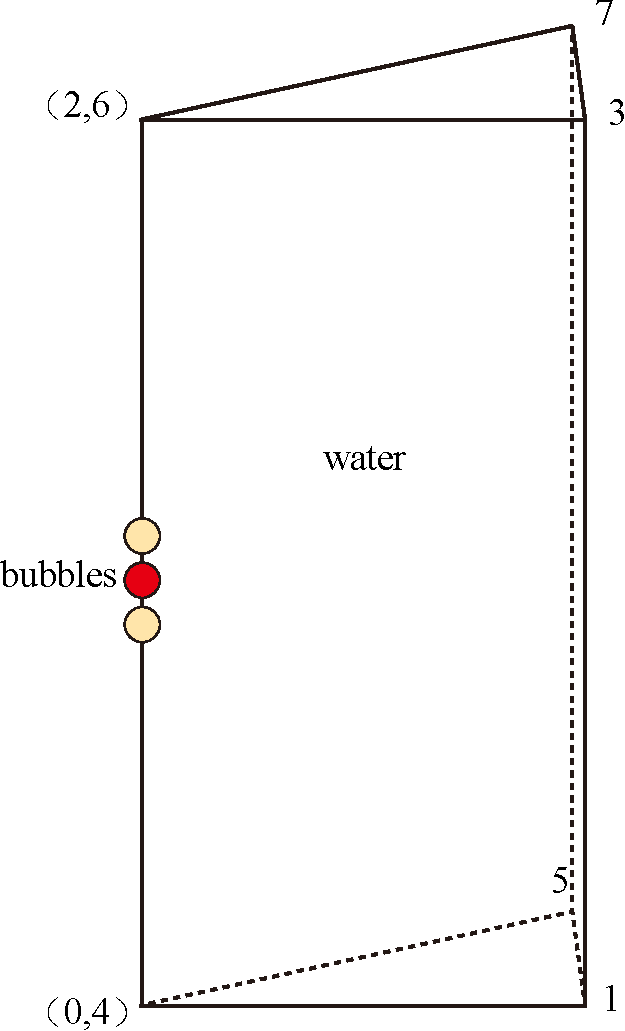
\includegraphics[width=0.4\linewidth]{img/fig2.8-eps-converted-to.pdf}
\centering
\caption[计算域]{在计算域中,(0, 2,
6, 4)设置为旋转对称周 symmetryPlane,底面 bottom(0, 1, 5, 4),顶面
top(2, 3, 7, 6),外面 outside(1, 3, 7, 5)属性是
patch,需要在具体情况中特殊定义,前后面 front(0, 1, 3, 2)、back(4, 5,
7, 6)是楔形对称面 wedge。}
\label{fig2.8}
\end{figure*}


具体的计算采用对称计算域,如图\ref{fig2.8}所示。其中对称面的角度
$\alpha=\mathrm{arctan} ((0.000016+0.000016)/0.005))=\mathrm{arctan} (0.0064)\approx 0.367^{\circ}$
。这样可以获得体积上近1000倍的简化。全计算域采用六边形结构化网格。无网格膨胀。通过改变边界条件和计算域内条件来实现不同场景。有限体积法的计算速度受核间通信速度和缓存大小影响较大。最终计算通过租用超算和自组AMD-EPYC平台服务器进行。

\section{本章小结}

本章主要梳理了本作中涉及到的实验方法、理论模型和数值方法。其中光学击穿采用两种消球差方法以获得较好的击穿效果。采用了两种方法捕捉空泡的形状动态。利用了DOE进行分光。利用撞击产生了冲击压力波。回顾了空泡动力学的两个经典模型。并基于OpenFOAM编写了求解流场守恒方程的求解器,以实现对空泡动力学的模拟。